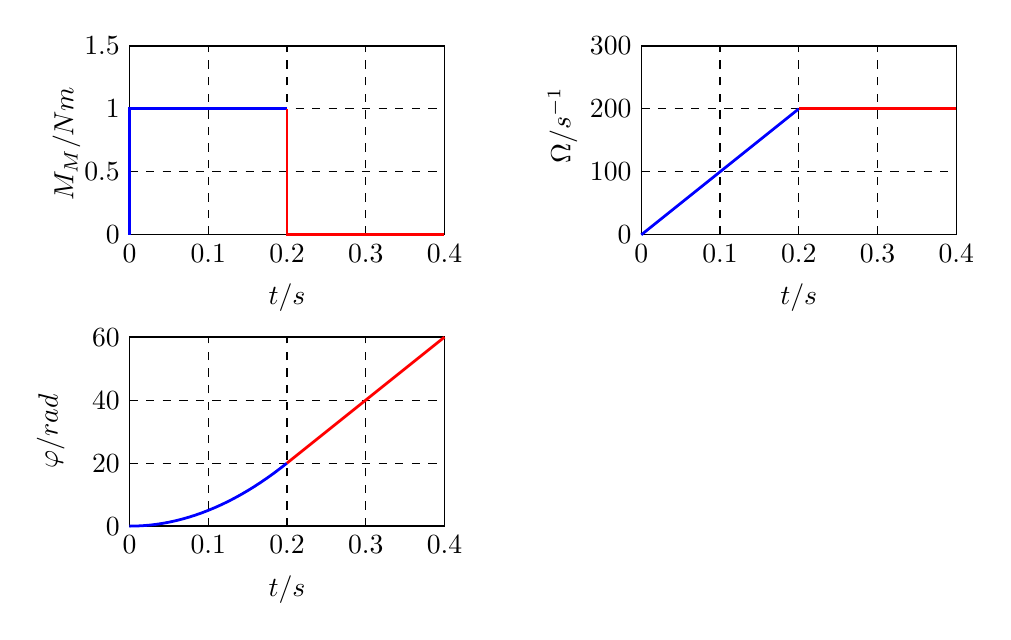
\begin{tikzpicture}
%
%Bewegungsprofil fuer J = 10e-4kgm^2
%
\draw[dashed,ystep=0.8] (0,0) grid (4,2.4);
\draw[line width = 0.5pt] (0,0) rectangle (4,2.4);
%
\draw(-0.8,2)node[left,rotate = 90]{$M_M/Nm$};
\foreach \y/\ytext in {0/0,0.8/0.5,1.6/1,2.4/1.5}
\draw(0,\y)node[left]{$\ytext$};
%
\draw(2,-0.5)node[below]{$t/s$};
\foreach \x/\xtext in {0/0,1/0.1,2/0.2,3/0.3,4/0.4}
\draw(\x,0)node[below]{$\xtext$};
%
%Drehmoment
%
\visible<2->{\draw[line width = 1pt,color = blue](0,0)--(0,1.6)--(2,1.6);}
\visible<3->{\draw[line width = 1pt,color = red](2,1.6)--(2,0)--(4,0);}
%
%--------------------------------------------------------------------
%
\begin{scope}[xshift = 6.5cm]
%
\draw[dashed,ystep=0.8] (0,0) grid (4,2.4);
\draw[line width = 0.5pt] (0,0) rectangle (4,2.4);
%
\draw(-1,2)node[left,rotate = 90]{$\Omega/s^{-1}$};
\foreach \y/\ytext in {0/0,0.8/100,1.6/200,2.4/300}
\draw(0,\y)node[left]{$\ytext$};
%
\draw(2,-0.5)node[below]{$t/s$};
\foreach \x/\xtext in {0/0,1/0.1,2/0.2,3/0.3,4/0.4}
\draw(\x,0)node[below]{$\xtext$};
%
%Omega
%
\visible<2->{\draw[line width = 1pt,color = blue](0,0)--(2,1.6);}
\visible<3->{\draw[line width = 1pt,color = red](2,1.6)--(4,1.6);}
%
\end{scope}
%
%--------------------------------------------------------------------
%
\begin{scope}[yshift = -3.7cm]
%
\draw[dashed,ystep=0.8] (0,0) grid (4,2.4);
\draw[line width = 0.5pt] (0,0) rectangle (4,2.4);
%
\draw(-1,1.8)node[left,rotate = 90]{$\varphi/\text{rad}$};
\foreach \y/\ytext in {0/0,0.8/20,1.6/40,2.4/60}
\draw(0,\y)node[left]{$\ytext$};
%
\draw(2,-0.5)node[below]{$t/s$};
\foreach \x/\xtext in {0/0,1/0.1,2/0.2,3/0.3,4/0.4}
\draw(\x,0)node[below]{$\xtext$};
%
%\varphi
%
\visible<2->{\draw[line width = 1pt,color = blue,domain = 0:2]plot
(\x,{25*0.8*(\x*\x/100)});} %Skalierung der y-Achse auf 0.8 ^=20
\visible<3->{\draw[line width = 1pt,color =red](2,0.8)--(4,2.4);}
%
\end{scope}
%
\end{tikzpicture}